\documentclass[12pt]{article}
\usepackage{amsmath}
\usepackage{amssymb}
\usepackage{geometry}
\usepackage{enumerate}
\usepackage{natbib}
\usepackage{float}%稳定图片位置
\usepackage{graphicx}%画图
\usepackage[english]{babel}
\usepackage{a4wide}
\usepackage{indentfirst}%缩进
\usepackage{enumerate}%加序号
\usepackage{multirow}%合并行
\title{\large UM-SJTU JOINT INSTITUTE\\Intro to Circuits\\(VE215)\\\ \\\ \\\ \\\ \\\ \\\ \\\ \\\ \\\ \\\ \\\
LABORATORY REPORT\\\ \\\ EXERCISE 3\\\ Transient Lab \\\ \\\ \\\ \\\ \\\ }
\author{Name: Pan Chongdan\\ID: 516370910121\\Group: 16}
\date{Date: \today}
\begin{document}
\maketitle
\newpage
\section{Introduction and Theoretical Background}
\subsection{Objectives}
\begin{enumerate}
\item Apply the theory on the step responses in first and second order circuits to series RC and RLC circuits.
\item Build a series RC circuit, observe its responses to input square wave signal of varied frequency, and explain them based on the theor
\begin{enumerate}
\item Relate the observed capacitor voltage and resistor voltage as functions of time to calculations.
\item Explain the changes of both output waveforms in response to the increase of the frequency of the input square wave signal.
\item Explain the amplitudes of the capacitor voltage and the resistor voltage related to the amplitude of the input square wave
\end{enumerate}
\item Build a series RLC circuit, observe the three types of its responses to input square wave signal, and relate them to the theory. For the under-damped/ over-damped/ critical damped response, compare the resistance in the circuit measured in the lab with the critical resistance calculated in the pre-lab.
\item Build the simplest second-order circuit, an LC tank, and observe oscillations.
\end{enumerate}
\subsection{Theoretical Background}
\subsubsection{First-order Circuits}
Theoretically, the transient responses in electric circuits are described by differential equations. The circuits, whose responses obey the first-order differential equation
$$\frac{\mathsf{d}x(t)}{\mathsf{d}t}+\frac{1}{\tau}\cdot x(t)=f(t)$$
are called $\mathbf{first-order circuits}$. Their responses are always monotonic and appear in the form of exponential form
$$x(t)=K_1\cdot e^{-\frac{t}{\tau}}+K_2$$
\par A first-order 	circuit includes the effective resistance $R$ and one energy-storage element, an inductor $L$, or a capacitor $C$.
\par In an RC circuit, the time constant is
$$\tau=RC$$
\par In an LC circuit, the time constant is 
$$\tau=\frac{L}{R}$$
\par The $\mathbf{fall time}$ of a signal is defined as the interval between the moment when the signal reaches 90\% and the moment when the signal reaches 10\% level. Note that the 10\% level is reached between $2\tau$ and $3\tau$. Approximately, you can assume the fall time $\approx$ 2.2 $\tau$. After $t=5\tau$, the exponent practically equals zero.
\subsubsection{Second-order Circuits}
Many circuits involve two energy-storing elements, both an inductor $L$ and a capacitor $C$. Such circuits require a second-order differential equation description.
$$\frac{\mathsf{d}^2x(t)}{\mathsf{d}t^2}+2\cdot\alpha\cdot\frac{\mathsf{d}x(t)}{\mathsf{d}t}+\omega_0^2\cdot x(t)=f(t)$$
thus they are called $\mathbf{second-order circuits}$.
\par We will consider only second-order circuits with one inductor and one capacitor. The differential equation includes two parameters: the damping factor $\alpha$ and the undamped frequency $\omega_0$ which are determined by the circuit and its components.
\par For example, in the series RLC circuit, which you will build and study in this lab,
$$\alpha=\frac{R}{2\cdot L},\omega_0=\frac{1}{\sqrt{L\cdot C}}$$
\par while in the parallel RLC circuit
$$\alpha=\frac{1}{2\cdot R\cdot C},\omega_0=\frac{1}{\sqrt{L\cdot C}}$$
\par Depending on the two parameters $\alpha$ and $\omega_0$, second-order circuits can exhibit three types of response.
\subsubsection{The Underdamped Response}
If $\alpha<\omega_0$
$$x(t)=e^{-\alpha t}(K_1cos(\omega t)+K_2sin(\omega t))$$
where $\omega=\sqrt{\omega_0^2-\alpha^2}$
The underdamped circuit response involves decaying oscillations, which may
last for many periods or for less than one period, depending on the damping
ratio $\xi=\frac{\alpha}{\omega_0}$, which for the series RLC circuit $\xi=\frac{R}{2L}\sqrt{LC}=\frac{R}{2}\cdot\sqrt{\frac{C}{L}}$. Varying the values of $R,L,C$, affects the damping ration $\xi$.
\subsubsection{The Critically Damped Response}
if $\alpha=\omega_0$
$$x(t)=e^{-\alpha t}(K_1+K_2t)$$
and the circuit has the critically damped response.
\par The critically damped response does not involve oscillations.
\par For the series RLC circuits,$\alpha=\omega_0$ corresponds to $\frac{R}{2L}=\frac{1}{\sqrt{LC}}$ or $R=R_{critical}=2\sqrt{\frac{L}{C}}$.
\par If $L=1mH and C=10nF,$ then $R_{critical}\approx 632\Omega.$
\subsubsection{The Overdamped Response}
If $\alpha>\omega_0$
$$x(t)=K_1\cdot e^{s_1t}+K_2\cdot e^{s_2t}$$
where $s_1=-\alpha+\sqrt{\alpha^2-\omega_0^2}$ and $s_2=-\alpha-\sqrt{\alpha^2-\omega_0^2}$
\par In the series RLC circuits, the overdamped solution is obtained if the resistance is larger than the critical resistance, such that $R>R_{critical}=2\cdot\sqrt{\frac{L}{C}}$
\par Notice that the larger resistance corresponds to the longer delay, and even
the faster decay has a much longer fall time than the critically damped response.
\par One of the most interesting features of series RLC circuits is that increasing
the resistance above the critical value results in much longer fall time, or longer
delays of responses in digital circuits. Among all monotonic responses, the
critically damped is the fastest.
\section{Procedure}
\subsection{First-order Circuit}
\begin{enumerate}
\item \begin{enumerate}
\item I turned on the function generator, set a square wave at 1 $V_{ppk}$ and 100 Hz, and applied it to the circuit as the input signal.
\item I monitored the input signal in Channel 1 and the output in Channel 2 of the oscilloscope .
\end{enumerate}
\item For the For the fastest circuit response, set $R_P$=0, and set the oscilloscope:
\begin{enumerate}
\item Vertical scale for the input signal 200mV/div
\item Vertical scale for the output signal 200mV/div
\item Horizontal scale 5ms/div
\end{enumerate}
\item For the slowest circuit response, set 𝐑𝐏 = 10 kΩ, and set the oscilloscope:
\begin{enumerate}
\item Vertical scale for the input signal 200mV/div
\item Vertical scale for the output signal 50mV/div
\item Horizontal scale 5ms/div
\end{enumerate}
\end{enumerate}
\subsection{Second-order Circuit}
\begin{enumerate}
\item I set a square wave at 1$V_{ppk}$ and 10 kHz as the input signal on the function generator.
\item I varied $R_P$ to generate three kinds of plot on the oscilloscope.
\item I observed and saved the graph from the oscilloscope.
\item I record the fall time and rise time, the time interval between the neighbouring peaks, $\bigtriangleup t,$ and the resistance of the potentiometer, $R_P$.
\end{enumerate}
\section{Results}
\subsection{First-order Circuit}
\begin{table}[H]
\centering
\begin{tabular}{|c|c|}
\hline
$R_1$ & $C$ \\ \hline
1$k\Omega$ &$0.1\mu F$  \\ \hline
\end{tabular}
\caption{Resistance and capacitance}
\end{table}
\begin{table}[H]
\centering
\begin{tabular}{|c|c|c|}
\hline
The setting of the potentiometer & Fastest circuit response & Slowest circuit response  \\ \hline
$V_{ppk}$ of the input square wave[V]&1.09 & 1.11 \\ \hline
$V_{ppk}$ of the output square wave[V]&1.09& 1.05 \\ \hline
Period of the input square wave, T[ms]& 10.000 & 10.000 \\ \hline
Rise time of the output waveform,[ms]&0.219&2.344\\ \hline
Fall time of the output waveform,[[ms]&0.21&2.218  \\ \hline
\end{tabular}
\caption{Table for first-order circuit}
\end{table}
\subsection{Second-order Circuit}
\begin{table}[H]
\centering
\begin{tabular}{|c|c|}
\hline
$R_2$ & $100\Omega$ \\ \hline
$R_P$ &$10k\Omega$  \\ \hline
$L$ & $1mH$ \\ \hline
$C$ &$820pF$  \\ \hline
\end{tabular}
\caption{Resistance, inductance, and capacitance}
\end{table}
% Please add the following required packages to your document preamble:
% \usepackage{multirow}
\begin{table}[H]
\centering
\begin{tabular}{|c|c|c|c|c|}
\hline
                  &Resistance, $R_P$  &Rise time $[ms]$&Fall time $[ms]$&time interval $\bigtriangleup t$  \\ \hline
\multirow{2}{*}{}Under-damped &639  &$1.236\times 10^{-3}$&$1.208]times10^{-3}$&$99.99\times 10^{-3}$  \\ \cline{2-5} 
                  &1000  &$1.416\times 10^{-3}$& $1.416\times 10^{-3}$ &$100.0\times 10^{-3}$  \\ \hline
     critically damped & 2109&$2.704\times 10^{-3}$&$2.772\times10^{-3}$& \\ \hline
\multirow{2}{*}{}Over-damped &3113  &$4.668\times10^{-3}$ &$4.628\times10^{-3}$  &  \\ \cline{2-5} 
                  &4113  &$6.208\times10^{-3}$&$6.296\times10^{-3}$  &  \\ \hline
\end{tabular}
\caption{Table for second-order circuit}
\end{table}
\subsection{Graphs from waveform}
\begin{figure}[H]
\centering
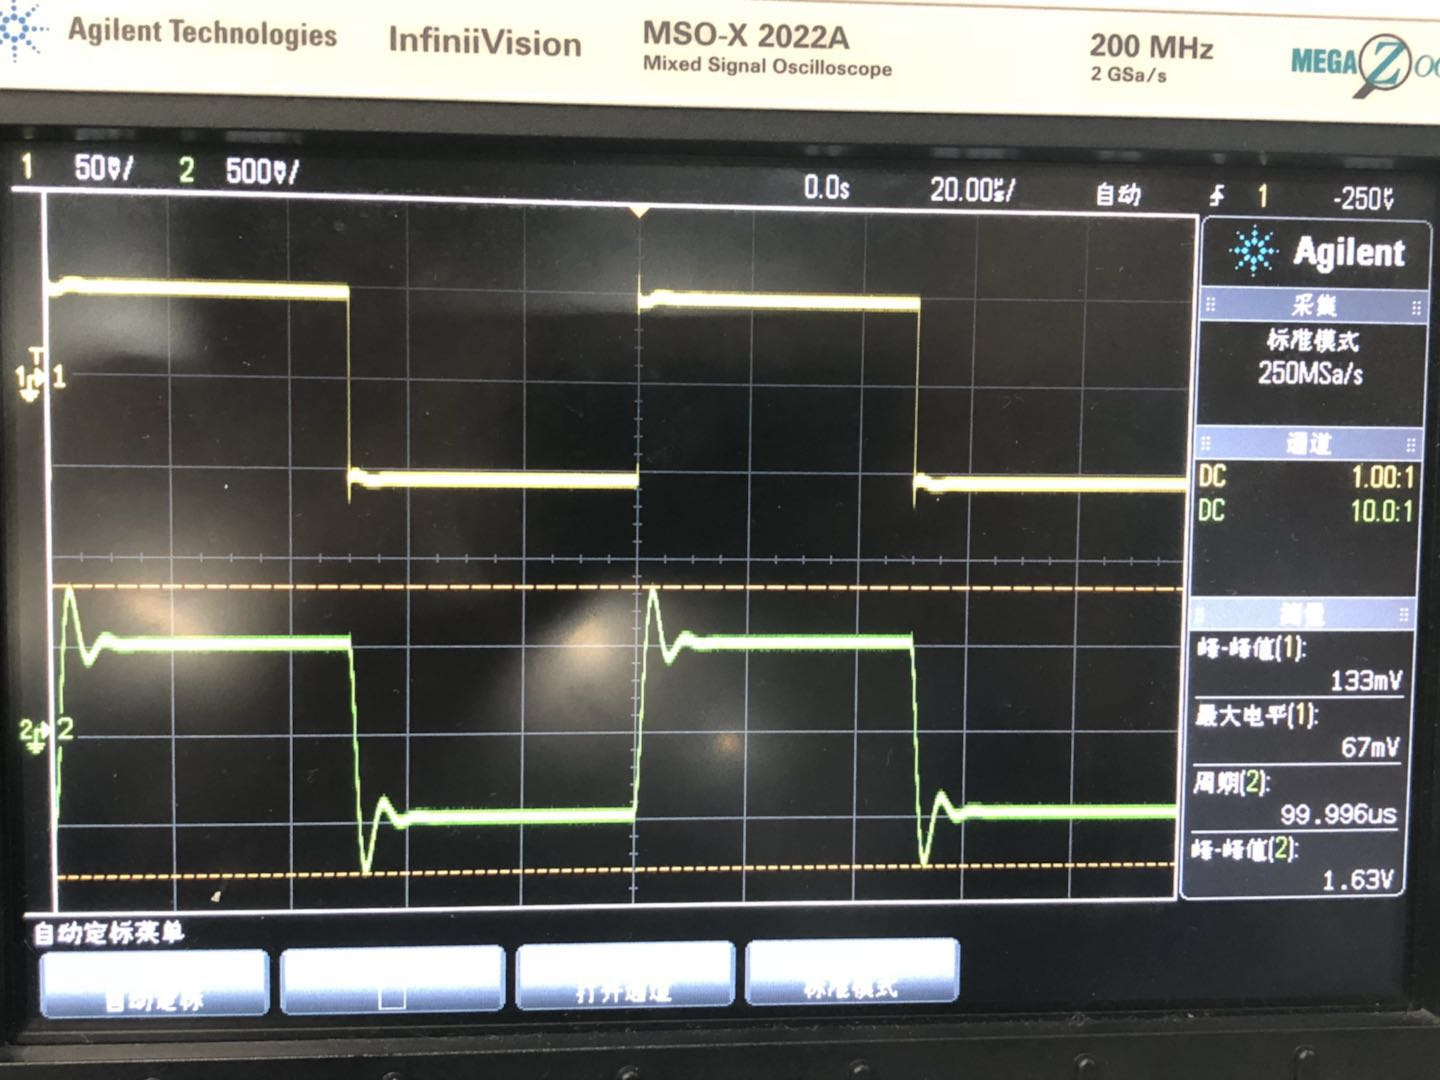
\includegraphics[scale=0.2]{P1.jpg}
\caption{Under-damped waveform when $R_P=639\Omega$}
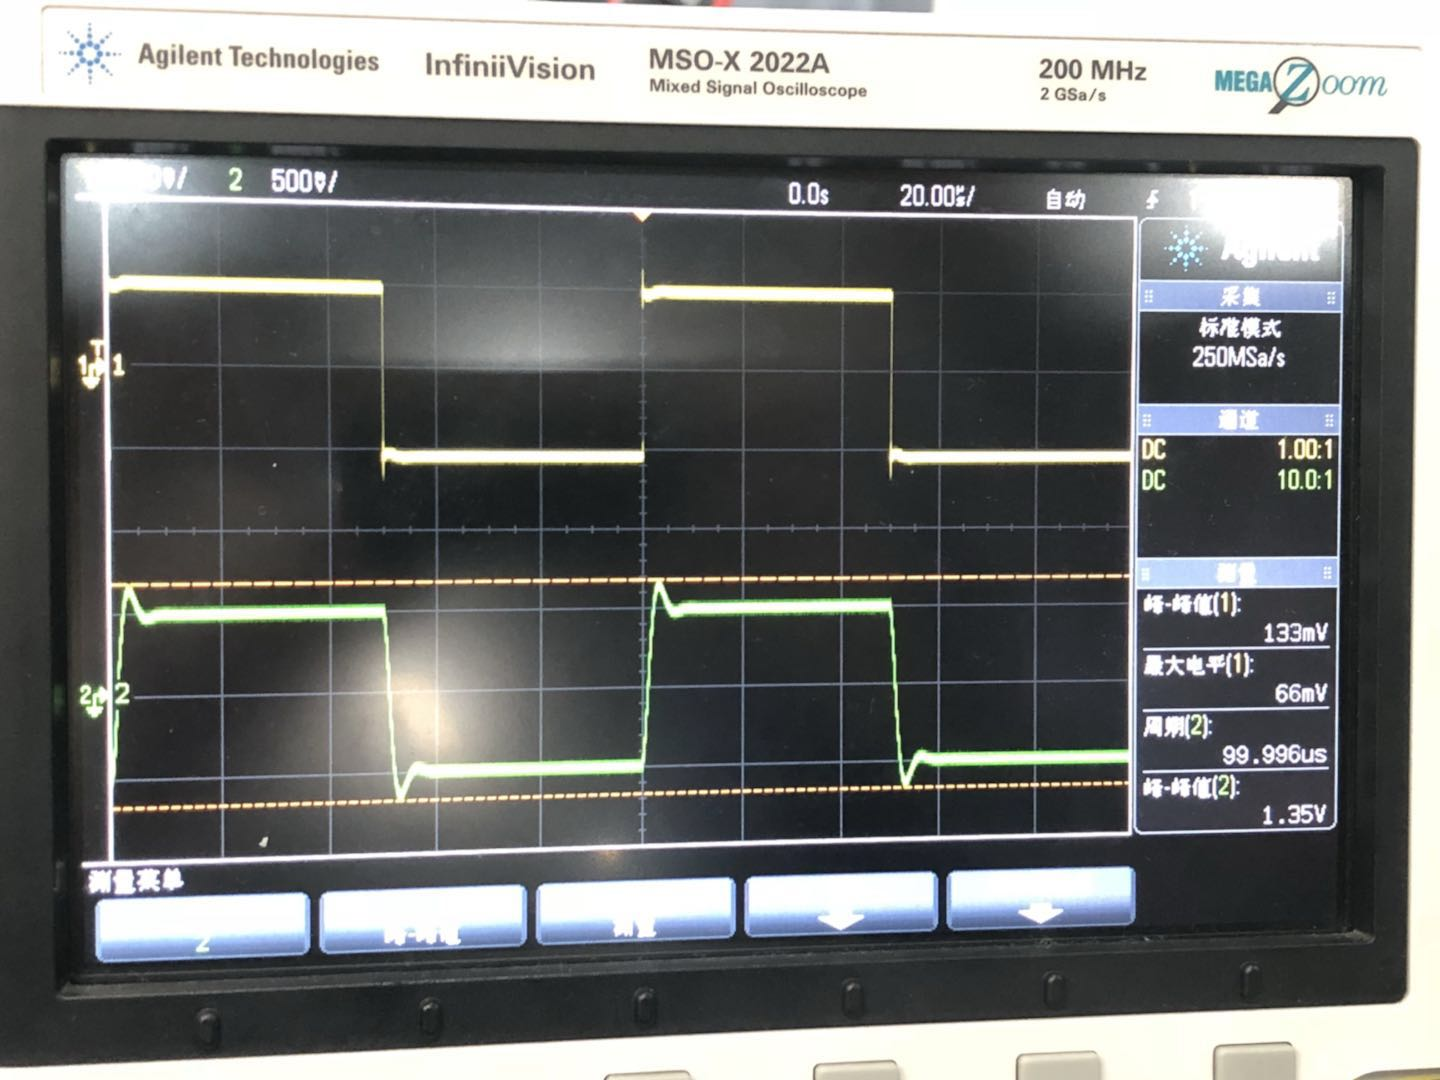
\includegraphics[scale=0.2]{P2.jpg}
\caption{Under-damped waveform when $R_P=100\Omega$}
\end{figure}
\begin{figure}[H]
\centering
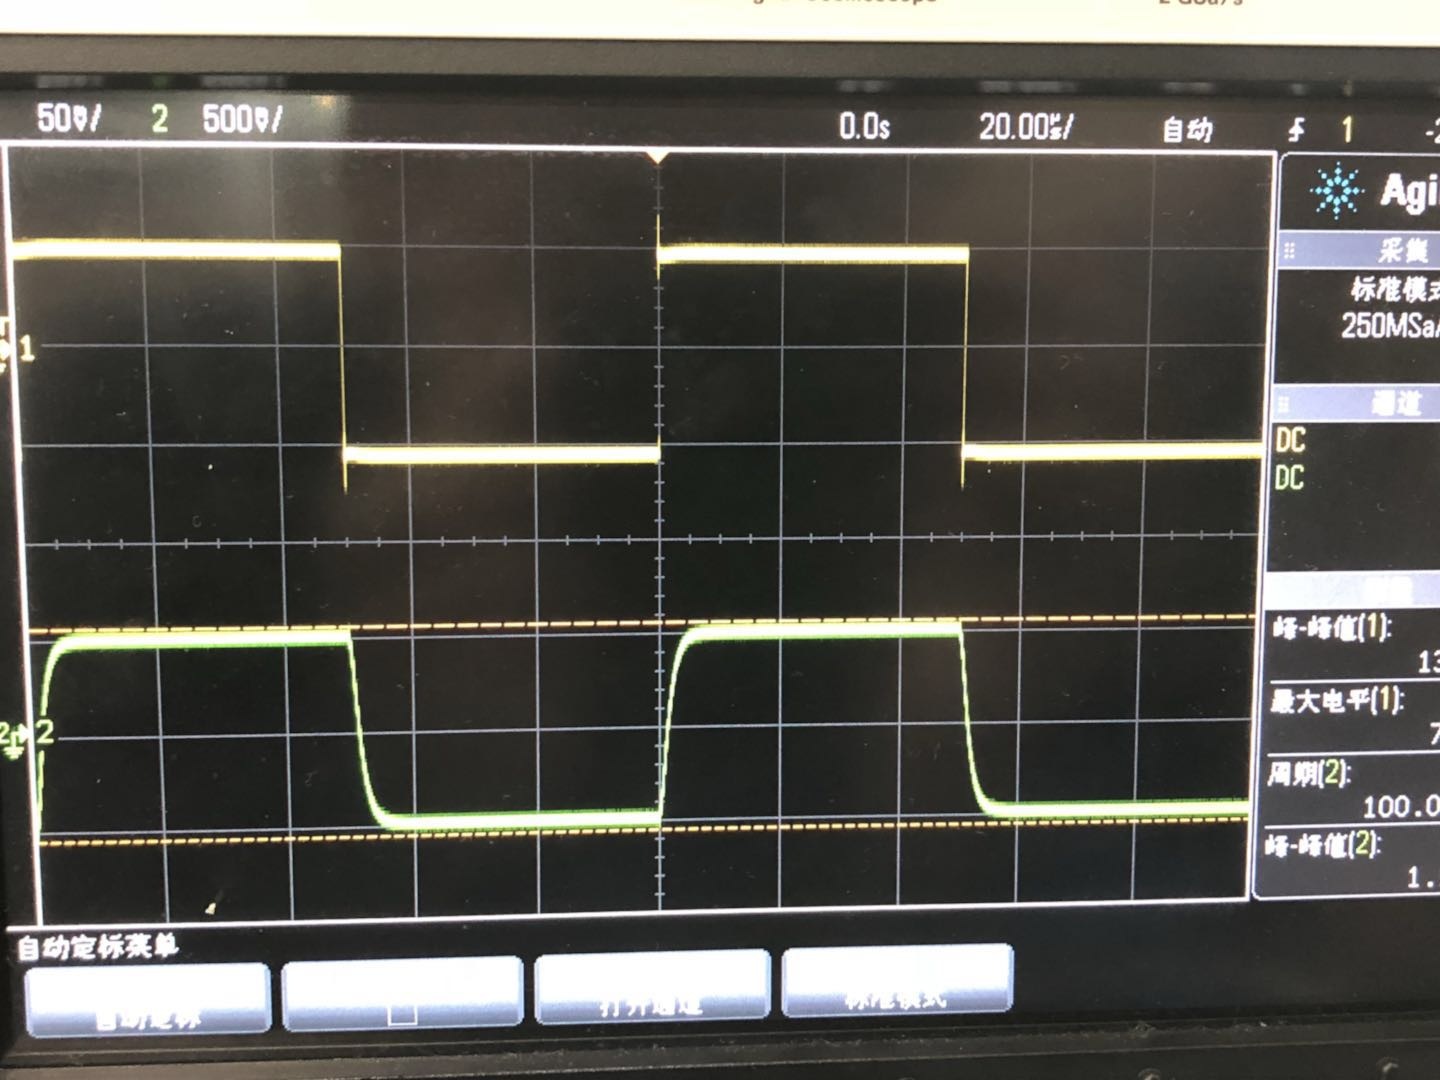
\includegraphics[scale=0.2]{P3.jpg}
\caption{Critically damped waveform when $R_P=2109\Omega$}
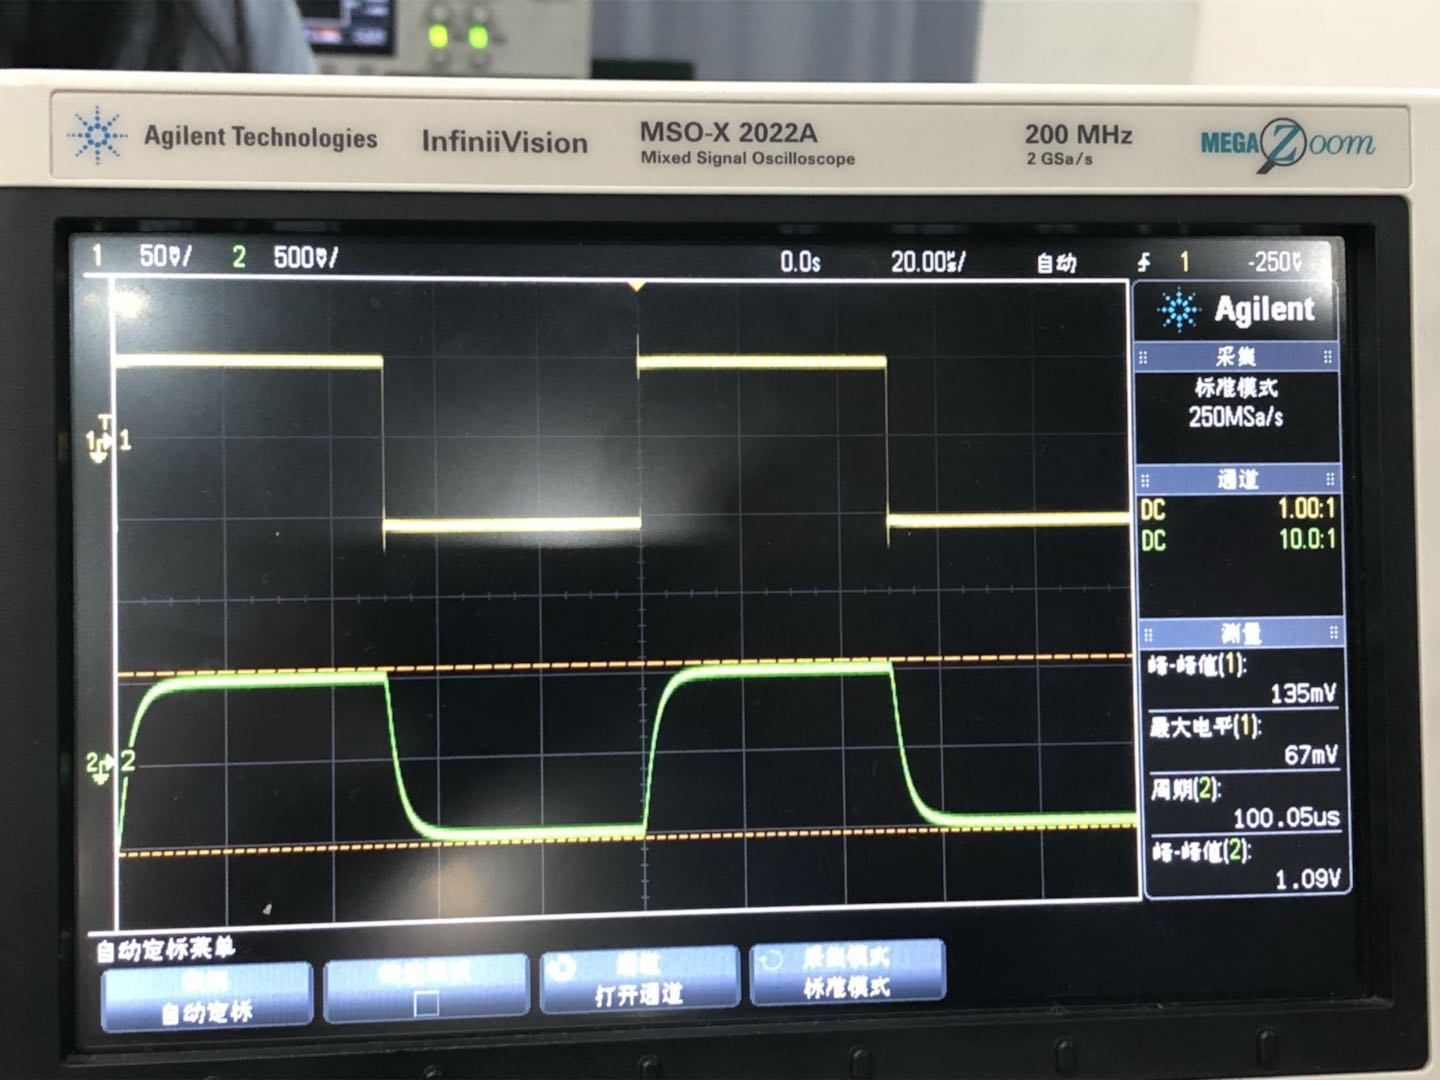
\includegraphics[scale=0.2]{P4.jpg}
\caption{Over-damped waveform when $R_P=3113\Omega$}
\end{figure}
\begin{figure}[H]
\centering
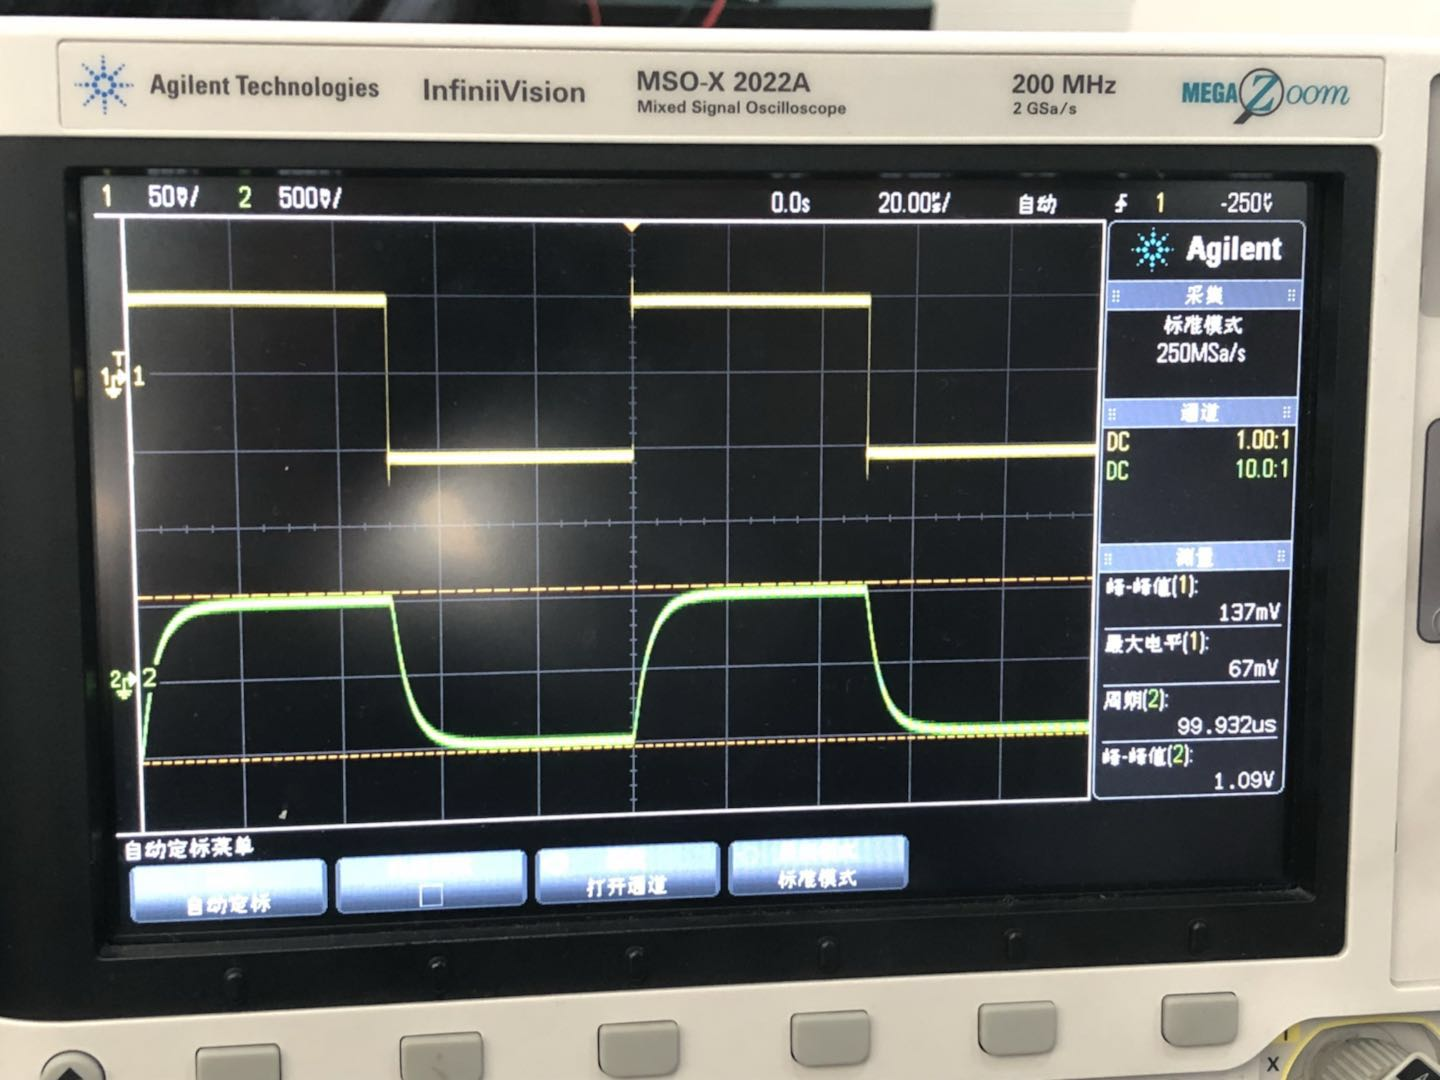
\includegraphics[scale=0.2]{P5.jpg}
\caption{Over-damped waveform when $R_P=4113\Omega$}
\end{figure}
\section{Conclusion}
In this lab work, I built series $RC$ and $RLC$ circuits, and studied the step responses on these corresponding first-order and second-order circuits.
\par For the first-order circuit, I measured the rise time and fall time when the circuit has fastest response and slowest response respectively. With the increase of $R_P$ the rise time and fall time is also increasing.
\par When $R_P=0[\Omega]$, which means the circuit has the fastest response, the $V_{ppk}$ of input square wave and output square wave is very close, which is $1.09[V]$. The period of the input square wave $T=10[ms]$, which is equal to the theoretical value $\frac{1}{100\cdot 1000}=0.01[s]$. According to the pre-lab assignment, I calculated $\tau=1\cdot 10^{-4}[s]$, so the theoretical value of rise time and fall time is $2.2\tau=2.2\cdot10^{-4}[s]$, which is very similar to my measured value: $0.219[ms]$ and $0.210[ms]$.
\par When $R_P=10[k\Omega]$, which means the circuit has the fastest response, the $V_{ppk}$ of input square wave and output square wave is not as close as fastest response, which is $1.05[V]$ and $1.11[V]$. The period of the input square wave $T=10[ms]$, which is equal to the theoretical value $\frac{1}{100\cdot 1000}=0.01[s]$. According to the pre-lab assignment, I calculated $\tau=1.1\cdot 10^{-3}[s]$, so the theoretical value of rise time and fall time is $2.2\tau=2.42\cdot10^{-3}[s]$, which is very similar to my measured value: $2.344[ms]$ and $2.218[ms]$.
\par For the second-order circuit, I also measure the rise time and fall time during under-damped, critically damped, and over-damped conditions. Similar to first-order circuit, the rise time and  fall time also becomes bigger as $R_P$ increasing.
\par In pre-lab assignment, I'm asked to use $PSpice$ to build the first-order and second-order circuit to stimulate the waveform, and the results are similar to what I get from the screen. 
\section{Reference}
\begin{enumerate}[-]
\item \emph{VE215FA2017 Transient LabManual} 
\item \emph{Circuits Make Sense}, Alexander Ganago, Department of Electrical Engineering and Computer Science, University of Michigan, Ann Arbor.
\end{enumerate}
\end{document}